\documentclass{minimal}

\usepackage{tikz}
\usetikzlibrary{
	arrows.meta,
	decorations.pathmorphing,
	backgrounds,
	positioning,
	fit,
	petri,
	shapes.misc,
	graphs,
	quotes,
	decorations.pathreplacing,
	calc,
}

%\input{tikz_styles.tex}  % styles used in figures
\tikzset{infectious/.style={
		% The shape:
		rectangle,rounded corners=2mm,
		% The size:
		minimum size=8mm,
		% The border:
		very thick,
		draw=red!50!black!50, % 50% red and 50% black,
		% and that mixed with 50% white
		% The filling:
		top color=white, % a shading that is white at the top...
		bottom color=red!50!black!20, % and something else at the bottom
		% make sure text aligns properly 
		text height=1.5ex,text depth=.25ex,
}}

\tikzset{noninfectious/.style={
		% The shape:
		rectangle,rounded corners=2mm,
		% The size:
		minimum size=8mm,
		% The rest
		very thick,draw=black!50,
		top color=white,bottom color=black!20,
		% make sure text aligns properly 
		text height=1.5ex,text depth=.25ex,
}}

\tikzset{supinfectious/.style={
		% The shape:
		rectangle,rounded corners=2mm,
		% The size:
		minimum size=9.5mm,
		% The border:
		very thick,
		draw=red!50!black!50, % 50% red and 50% black,
		% and that mixed with 50% white
		% The filling:
		top color=white, % a shading that is white at the top...
		bottom color=red!50!black!20, % and something else at the bottom
		% make sure text aligns properly 
		text height=1.5ex,text depth=.25ex,
}}

\tikzset{supnoninfectious/.style={
		% The shape:
		rectangle,rounded corners=2mm,
		% The size:
		minimum size=9.5mm,
		% The rest
		very thick,draw=black!50,
		top color=white,bottom color=black!20,
		% make sure text aligns properly 
		text height=1.5ex,text depth=.25ex,
}}

\tikzset{noninfectious/.style={
		% The shape:
		rectangle,rounded corners=2mm,
		% The size:
		minimum size=8mm,
		% The rest
		very thick,draw=black!50,
		top color=white,bottom color=black!20,
		% make sure text aligns properly 
		text height=1.5ex,text depth=.25ex,
}}

\begin{document}
	
	\pagestyle{empty}
	
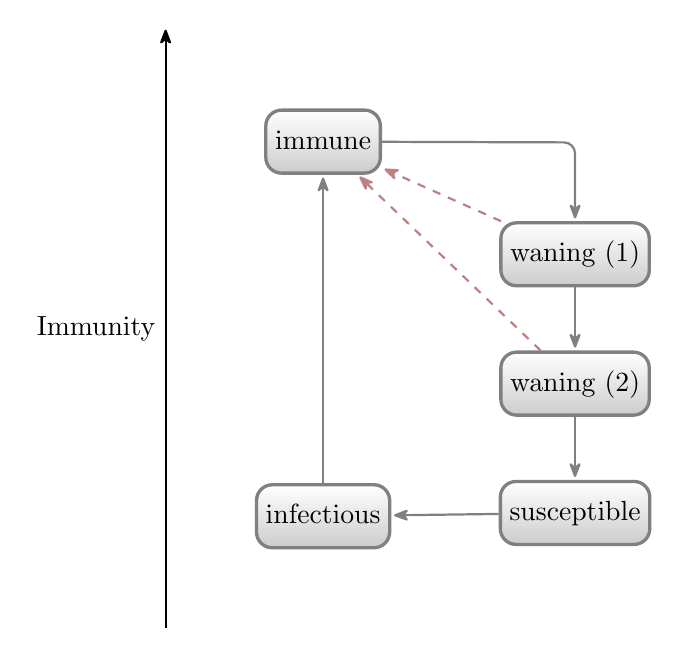
\begin{tikzpicture}[>={Stealth[round]},thick,black!50,text=black,
	every new ->/.style={shorten >=1pt},
	graphs/every graph/.style={edges=rounded corners}]
	\graph [grow down sep=8mm, branch right=7mm] {
		w1/"waning (1)" [noninfectious] ->
		w2/"waning (2)" [noninfectious] -> 
		susceptible [noninfectious] ->
		infectious [noninfectious, xshift=-32mm, yshift=16mm] ->
		immune [noninfectious, xshift=-32mm, yshift=80mm] 
		;
	};
	\draw [->,rounded corners,shorten >= 1pt,dashed,red!50!black!50,] (w1) -- (immune); 
	\draw [->,rounded corners,shorten >= 1pt] (immune) -- ($ (w1.north) + (0mm,10mm) $) -- (w1); 
	\draw [->,rounded corners,shorten >= 1pt,dashed,red!50!black!50,] (w2) -- (immune);
	\draw [->,thick,black] ($ (infectious.south) + (-20mm,-10mm) $) to [edge label=Immunity,color=black,] ($ (immune.north) + (-20mm,10mm) $);
\end{tikzpicture}

	
\end{document}



